%!TEX root = ../risk_report.tex

\chapter{A comparison of economics, health, and political risks}

In this chapter, we use subcorpora of economics, health and politics articles to understand how risk words change in specific semantic fields. Due to the smaller size of these subcorpora, we use different techniques

\section{~}

Key participants were first tallied (\texttt{/NN.?/ \textgreater \textgreater \# (NP !> PP)}) in order to broadly understand the key social actors in the three subcorpora (see Figure \ref{fig:clouds}).

			\begin{figure}[htb!]
			\centering
			\addvbuffer[12pt 8pt]{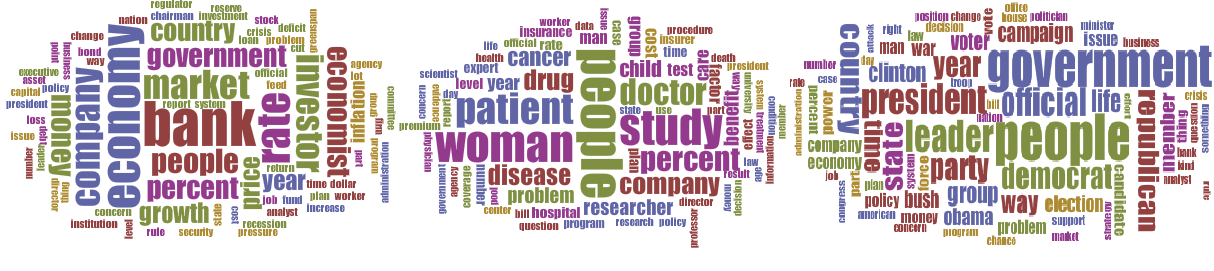
\includegraphics[width=0.75\textwidth]{../images/clouds.png}}
			\caption{Key participants in the \emph{Economics}, \emph{Health} and \emph{Politics} subcorpora}
			\label{fig:clouds}
			\end{figure}

			\begin{figure}[htb!]
			\centering
			\addvbuffer[12pt 8pt]{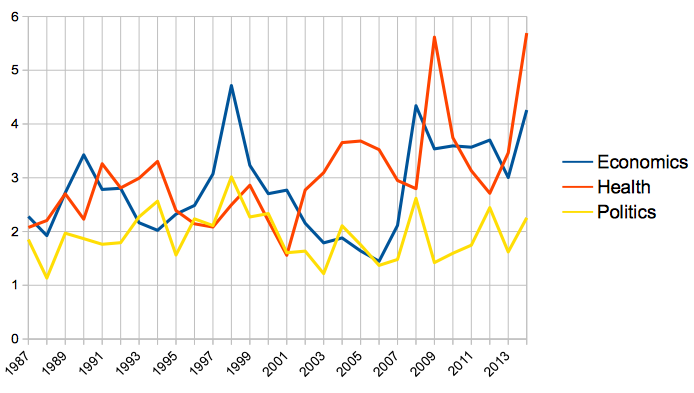
\includegraphics[width=.70\textwidth]{../images/echepol_riskwords.png}}
			\caption{Risk words per total number of article topics per year}
			\label{fig:echepol_riskwords}
			\end{figure}
			%
			Due to time constraints, we restricted the topic comparison to domains that had yielded interesting insights in the earlier interrogations. Further, we found that the smaller size of the subcorpora limited us to lexicogrammatical queries that outputted a large enough number of results for quantitative reliablity. Thus, we focussed on the following three areas:

		 	\begin{table}[htb!]
		 	\centering
		 	\small
		 	\begin{tabular}{|l|l|l|}
		 			 	\hline
		 			 	\textbf{Economics}   & \textbf{Health}         & \textbf{Politics}     \\ \hline
		 			 	political   & high           & political    \\ \hline
		 			 	big         & great          & great        \\ \hline
		 			 	economic    & low            & big          \\ \hline
		 			 	financial   & other          & high         \\ \hline
		 			 	great       & serious        & own          \\ \hline
		 			 	high        & financial      & serious      \\ \hline
		 			 	more        & potential      & new          \\ \hline
		 			 	real        & medical        & real         \\ \hline
		 			 	systemic    & more           & considerable \\ \hline
		 			 	significant & significant    & more         \\ \hline
		 			 	new         & cardiovascular & other        \\ \hline
		 			 	little      & political      & significant  \\ \hline
		 			 	global      & possible       & economic     \\ \hline
		 			 	serious     & small          & financial    \\ \hline
		 			 	other       & real           & potential    \\ \hline
		 			 	excessive   & such           & personal     \\ \hline
		 			 	potential   & genetic        & little       \\ \hline
		 			 	such        & ovarian        & such         \\ \hline
		 			 	much        & same           & public       \\ \hline
		 			 	own         & bad            & military     \\ \hline
		 			 	\end{tabular}
		 			 	\caption{Most common adjectives modifying nominal risks in the topic subcorpora}
		 			 	\label{tab:echepo_adjmod}
		 	\end{table}

\section{Health}

    Our topic subcorpora were much smaller than our main corpus. As a result, lexicogrammatical querying did not yield quantitatively reliable results. Accordingly, other kinds of corpus linguistic investigation, not reliant on grammatical structure, were applied. 

    First, we considered \emph{keywords}---that is, words that were unusually frequent within the health corpus when compared to the corpus as as a whole.

    Linear regression was used to determine the slope of each keyword's trajectory, and ensure that the p-value of this slope was below 0.05. Results were then sorted into two groups, based on the incline\slash decline of the slope.

    \noindent
    \begin{figure}[htb!]
    \centering
    \begin{minipage}{.45\textwidth}
    \centering
    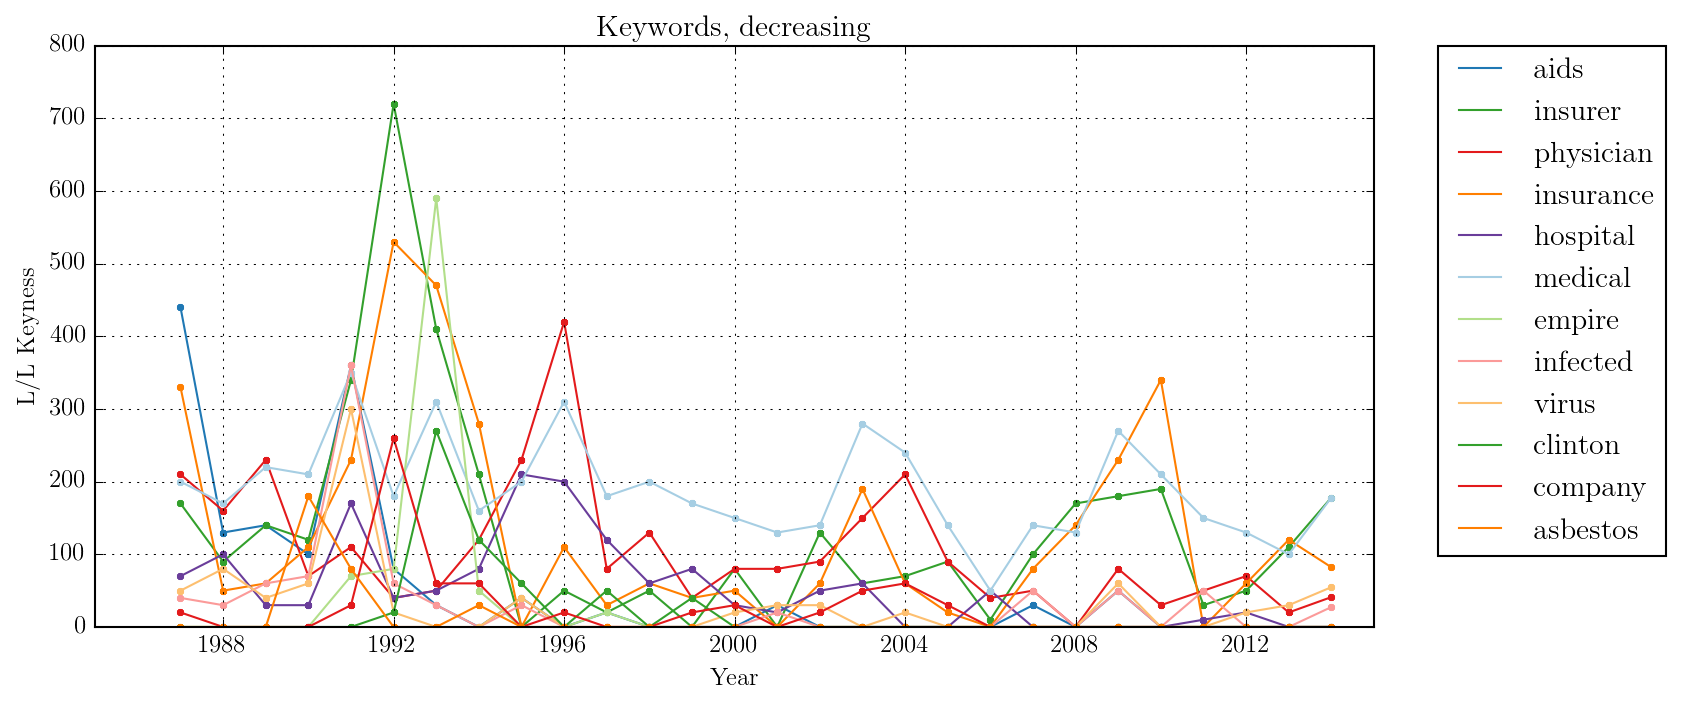
\includegraphics[width=.95\textwidth]{../images/keywords-decreasing.png}
    \caption{Keywords becoming more key over time}
    \label{fig:key-inc}
    \end{minipage}%
    \begin{minipage}{.55\textwidth}
    \centering
    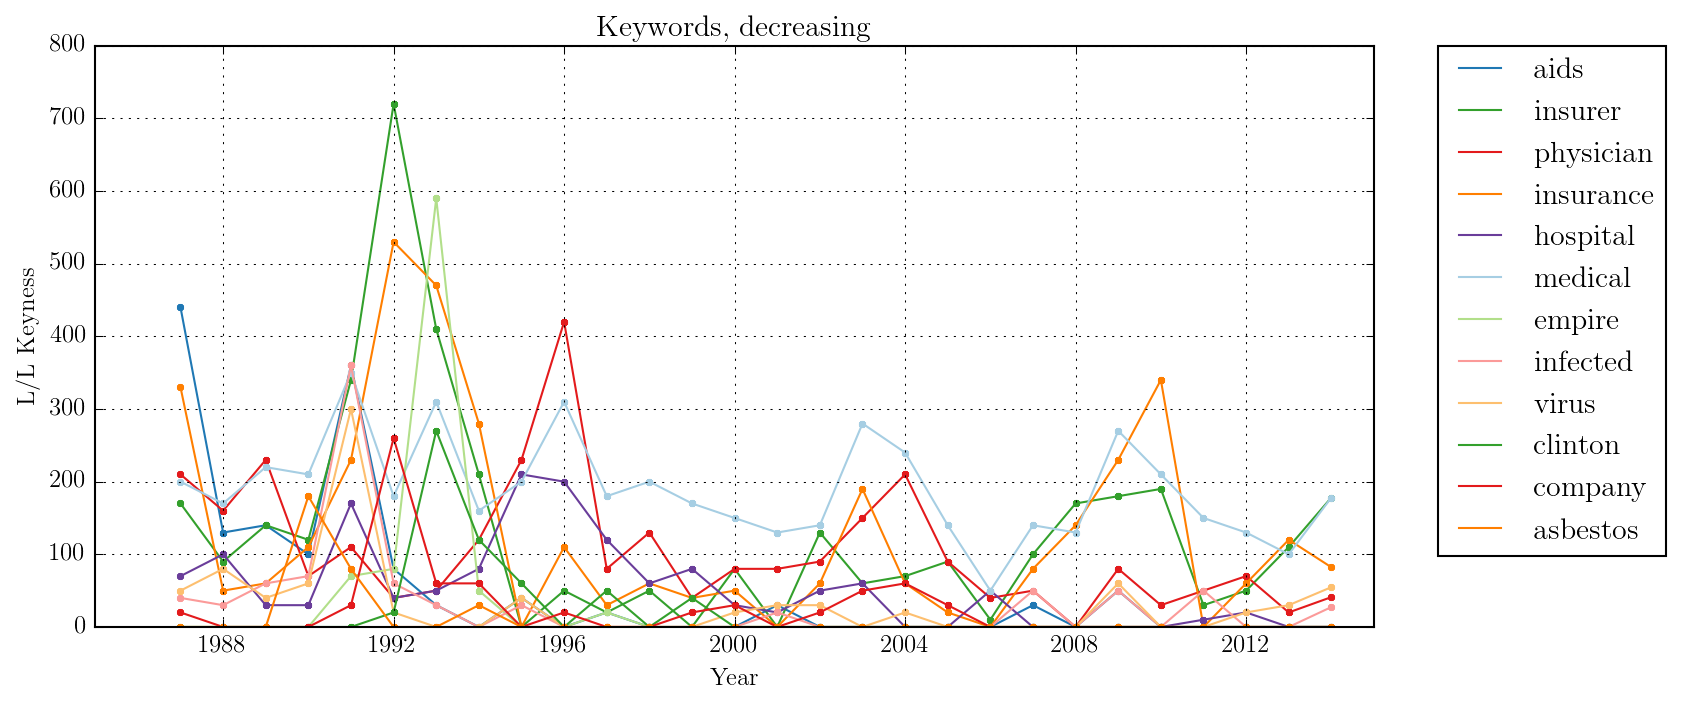
\includegraphics[width=.95\textwidth]{../images/keywords-decreasing.png}
    \caption{Keywords becoming less key over time}
    \label{fig:key-dec}
    \end{minipage}
    \end{figure}

    Next, we were interested in \emph{bi-grams}---that is, words that occur beside each other multiple times within a corpus. Bigrams containing a stopword were excluded from analysis, as these results were generally common clusters of closed class words (\emph{in the}, \emph{of a}, \emph{one day}, etc.). Again, linear regression was used to group results into increasing and decreasing groups.

    \noindent
    \begin{figure}[htb!]
    \centering
    \begin{minipage}{.45\textwidth}
    \centering
    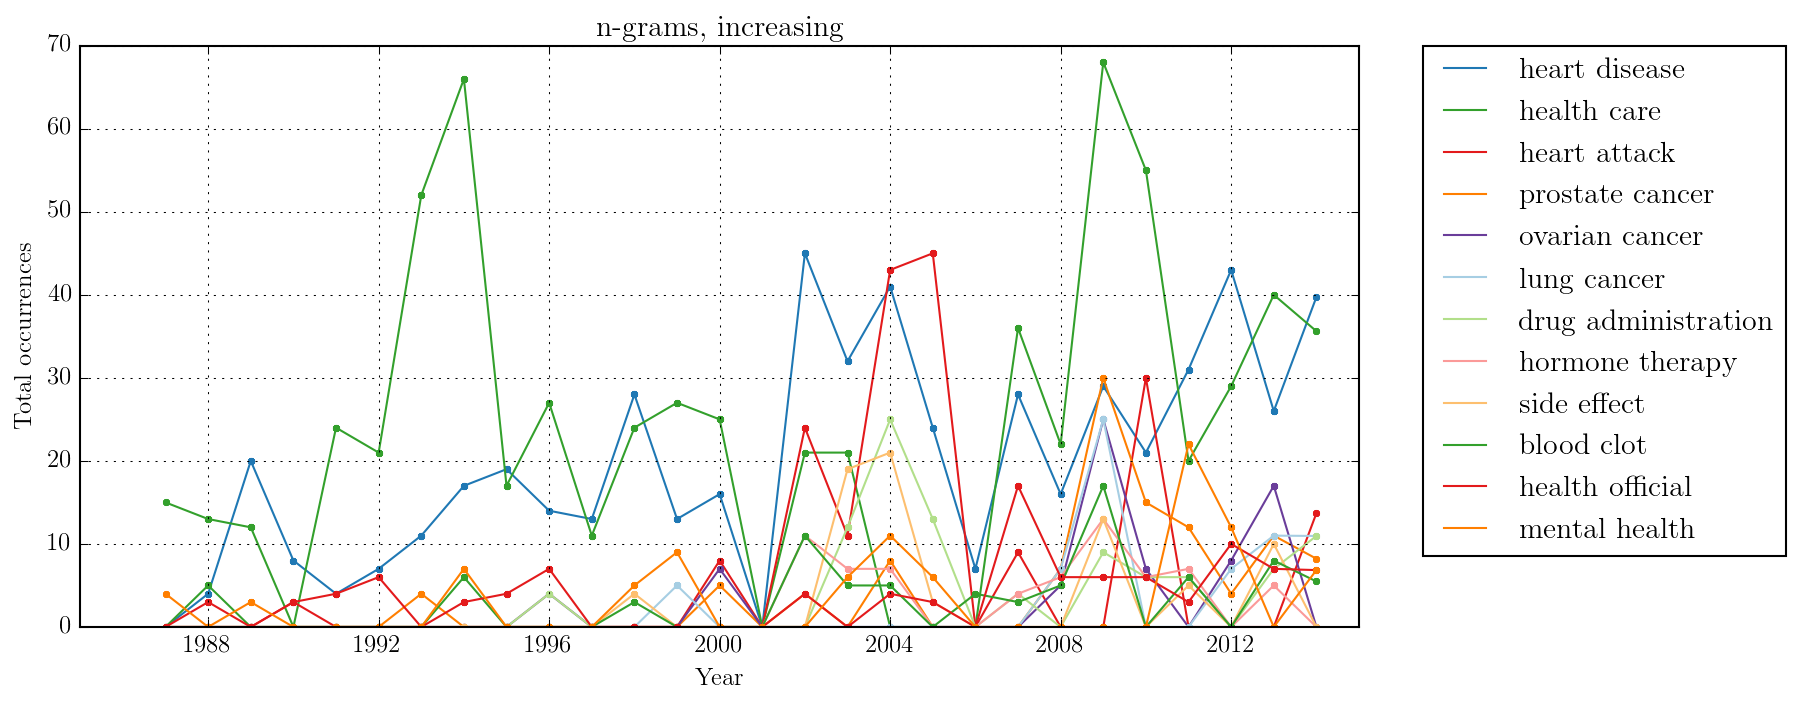
\includegraphics[width=.95\textwidth]{../images/ngrams-increasing.png}
    \caption{bi-grams becoming more frequent over time}
    \label{fig:ngram-inc}
    \end{minipage}%
    \begin{minipage}{.55\textwidth}
    \centering
    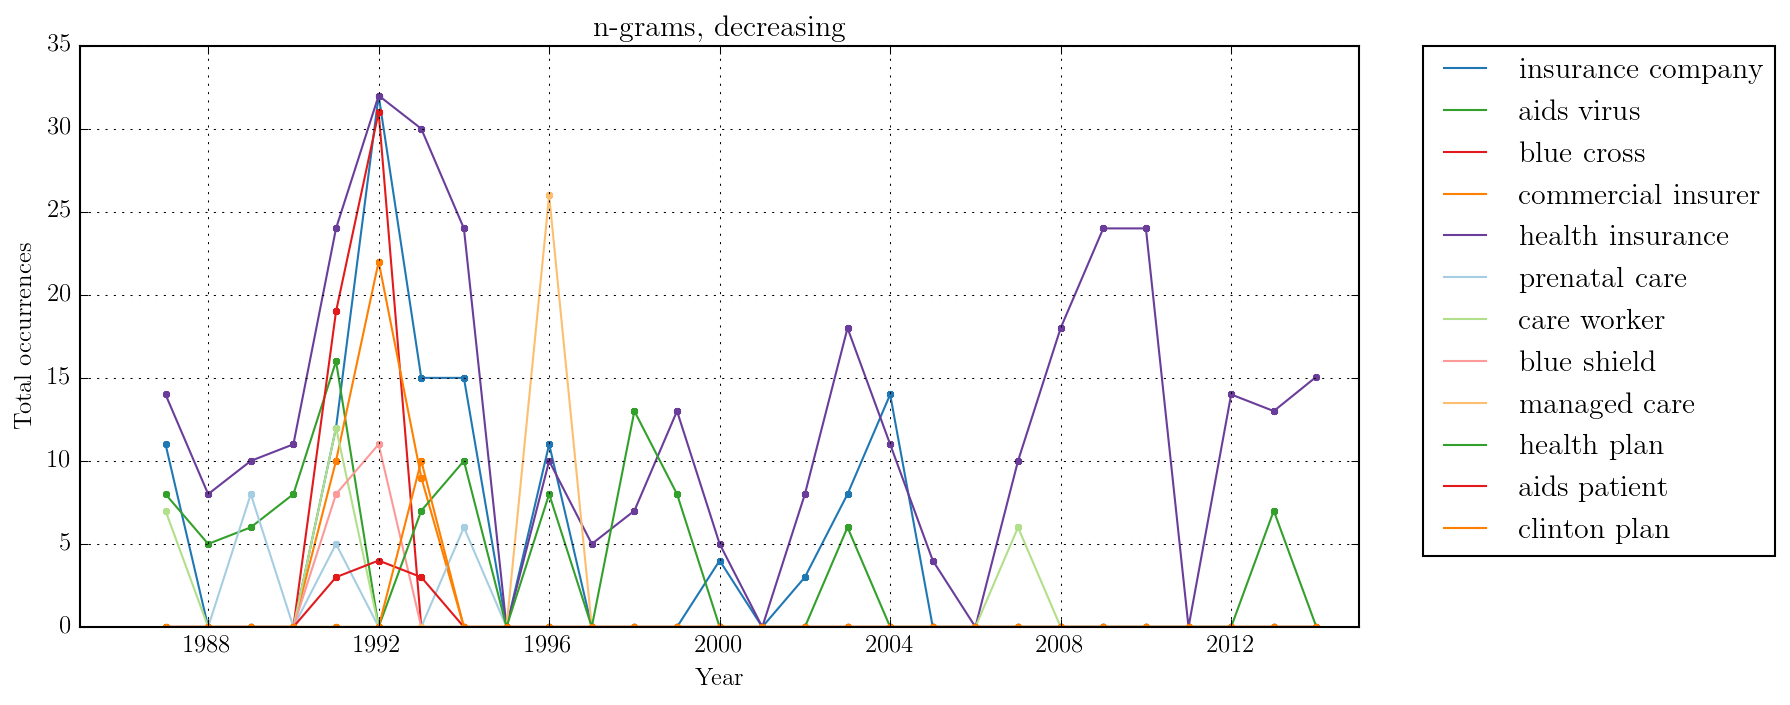
\includegraphics[width=.95\textwidth]{../images/ngrams-decreasing.png}
    \caption{bi-grams becoming less frequent over time}
    \label{fig:ngram-dec}
    \end{minipage}
    \end{figure}

We grouped these into themes, with results entered into one or more categories. Ambiguous results were often concordanced in order to determine the main context of use: \emph{athlete}, for example, could indicate the health condition (\emph{Athlete's foot}), a chain of footwear stores, or denote athletes themselves. The latter was revealed to be by far the most common context, and athlete was thus added to \emph{People, everyday}.

\section{Issues in the health corpus investigation}

The first major issue was the smaller size of the corpus, which necessitated different kinds of analysis.

Within keywording and ngramming, it became clear that broader linguistic change and specific events are difficult to separate.

This, however, is where we can see the clearest examples of the link between events and language change. Interspersed throughout the keywords and n-grams are terms ranging in specificity. It is through categorisation of these varying levels that we can smooth out the 

The keywording in particular revealed a number of ambiguities. A more reliable\slash systematic method for grouping keywords would ameliorate this concern.

\section{Summary}

	The smaller size of topic subcorpora necessitated different kinds of analysis. Fortunately, such methods are well documented within corpus assisted discourse studies. Following on from these methodologies, we located particularly frequent terms, and analysed them in their context of use.

	% analysis here

	Ultimately, the ways in which a corpus can be analysed are dependent on the size of the corpus. 



%\bibliography{../references/libwin}